\section{Visualizations on truncated Gaussian distribution}
\label{appendix:gaussian}

In this section we provide visual intuition for the source‐level sampling prior by plotting the truncated Gaussian density \(p(r\mid s)\) on the interval \([0,1]\) for a variety of center values \(s\) and scales \(\sigma\). Figures~\ref{fig:trunc_gauss_sigma_0.1},~\ref{fig:trunc_gauss_sigma_0.05},  and~\ref{fig:trunc_gauss_sigma_0.01} illustrate how annealing \(\sigma\) concentrates the distribution around its mean.

%—— figure for σ=0.1 ——%
\begin{figure}[!htbp]
  \centering
  \begin{tabular}{ccc}
    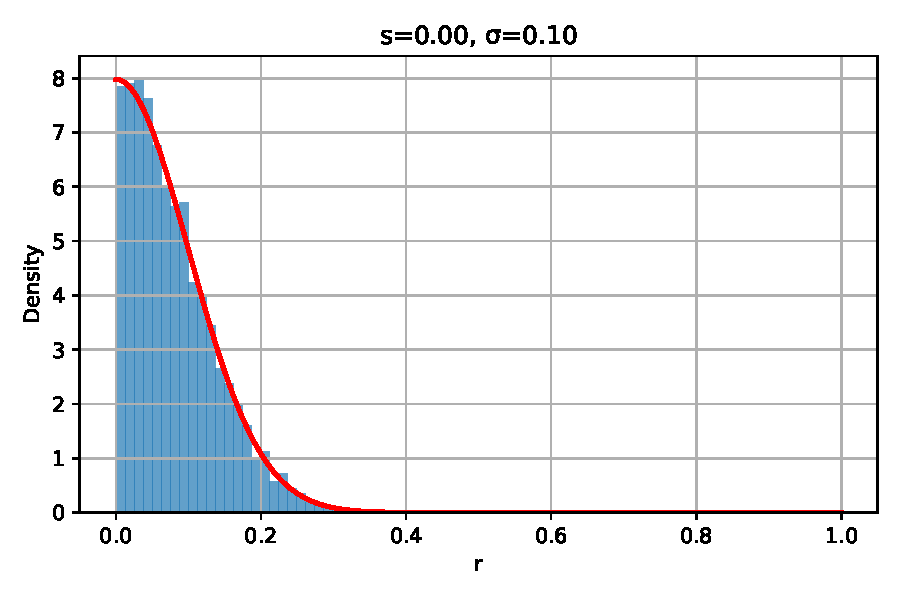
\includegraphics[width=0.32\linewidth]{pics/sampler/s00_step0.pdf} &
    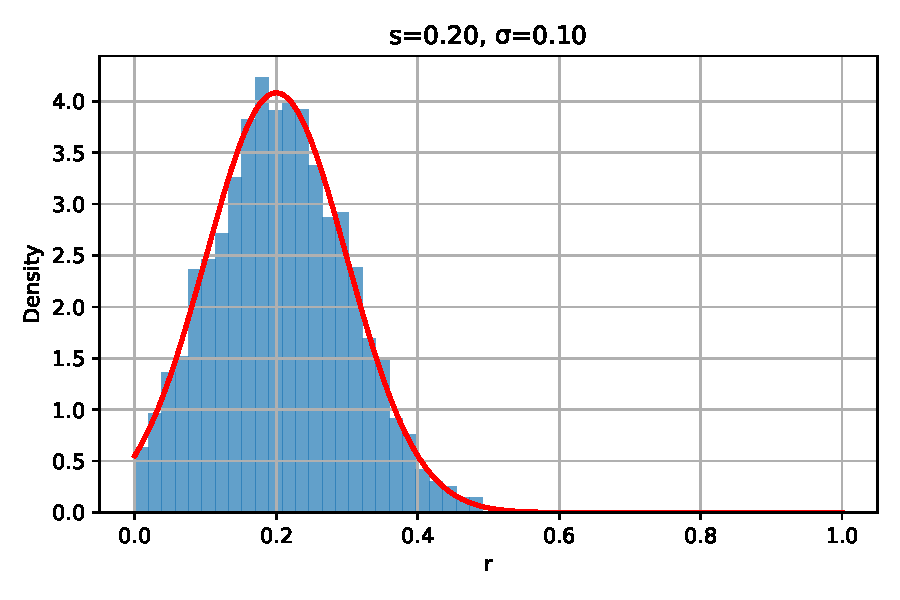
\includegraphics[width=0.32\linewidth]{pics/sampler/s20_step0.pdf} &
    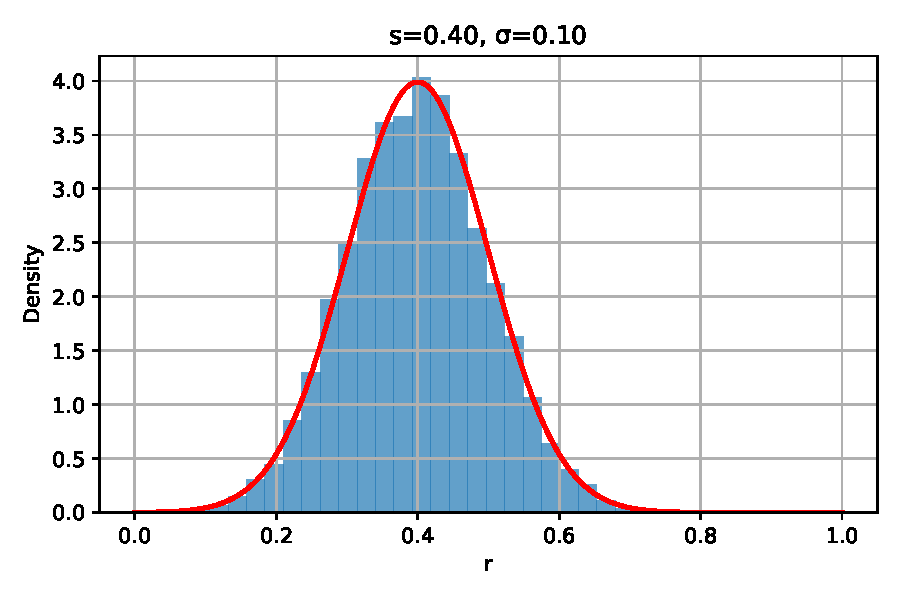
\includegraphics[width=0.32\linewidth]{pics/sampler/s40_step0.pdf} \\
    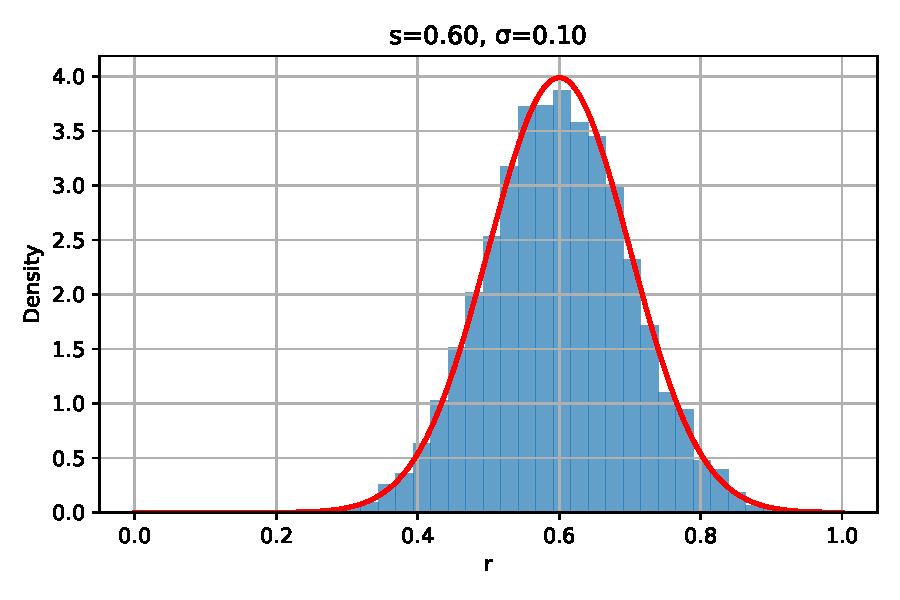
\includegraphics[width=0.32\linewidth]{pics/sampler/s60_step0.pdf} &
    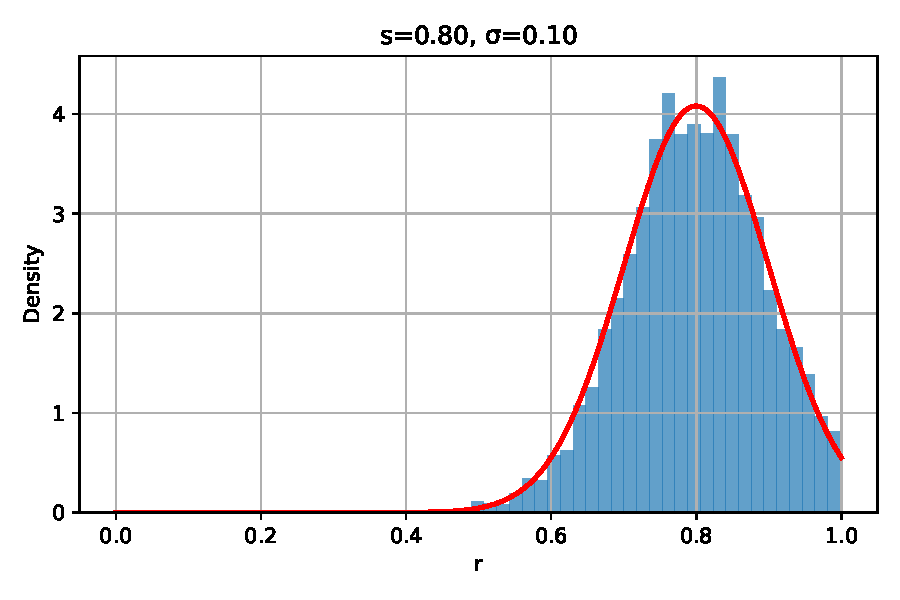
\includegraphics[width=0.32\linewidth]{pics/sampler/s80_step0.pdf} &
    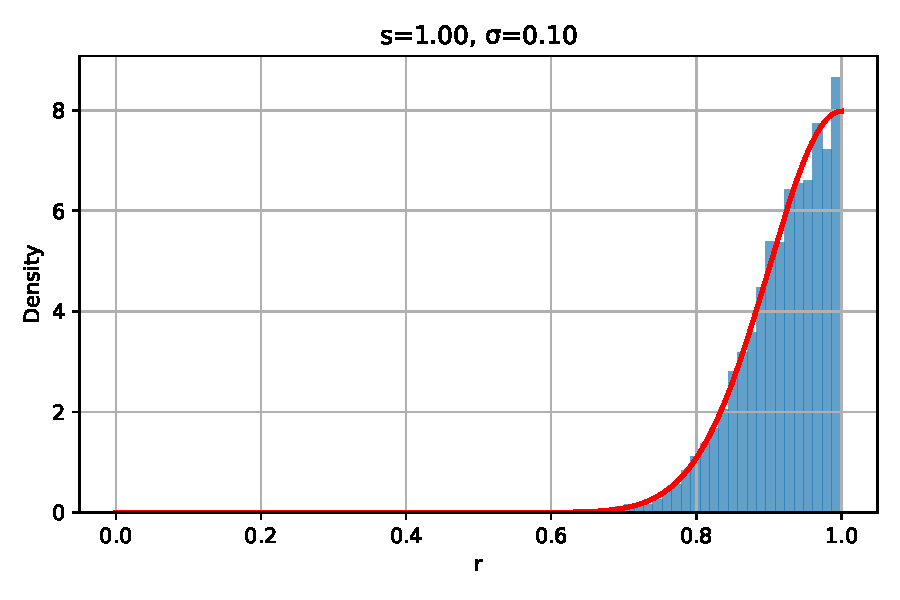
\includegraphics[width=0.32\linewidth]{pics/sampler/s100_step0.pdf} \\
  \end{tabular}
  \caption{Sampling prior \(p(r\mid s)\) on \([0,1]\) for various center values \(s\) with scale \(\sigma=0.1\).}
  \label{fig:trunc_gauss_sigma_0.1}
\end{figure}

%—— figure for σ=0.05 ——%
\begin{figure}[!htbp]
  \centering
  \begin{tabular}{ccc}
    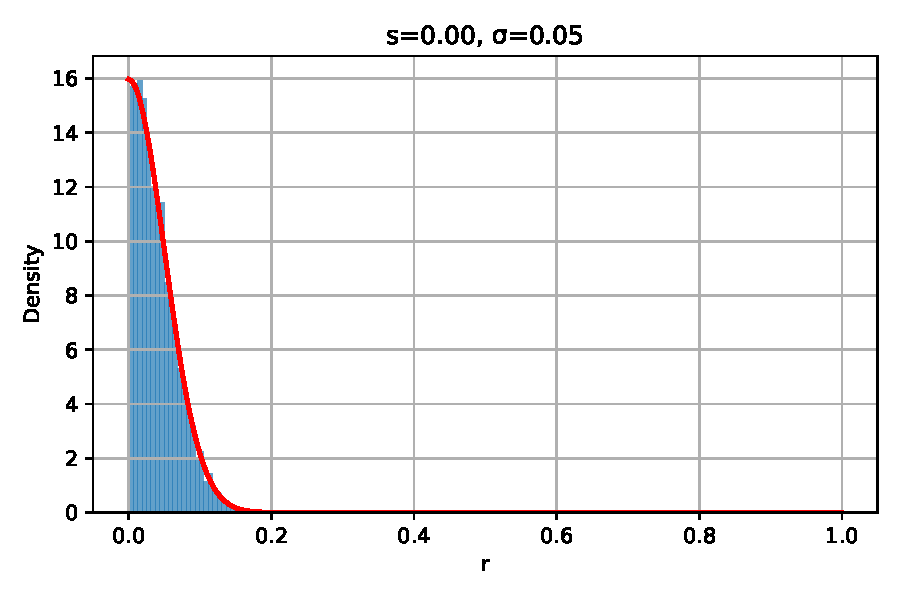
\includegraphics[width=0.32\linewidth]{pics/sampler/s00_step69.pdf} &
    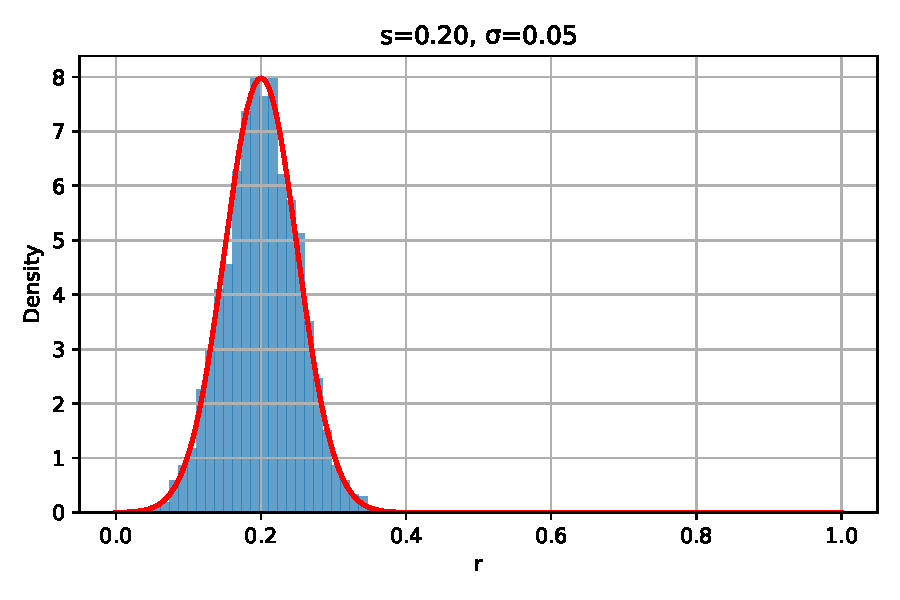
\includegraphics[width=0.32\linewidth]{pics/sampler/s20_step69.pdf} &
    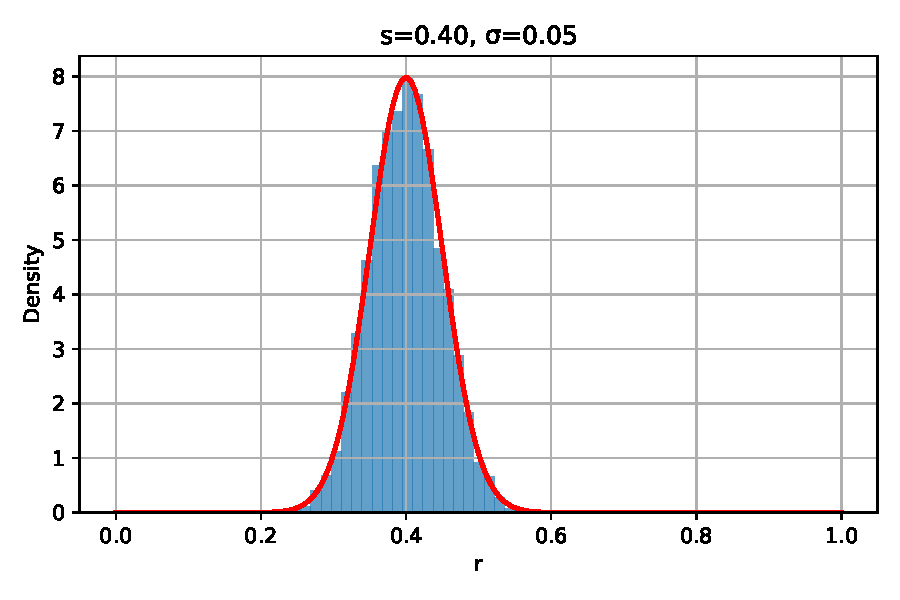
\includegraphics[width=0.32\linewidth]{pics/sampler/s40_step69.pdf} \\
    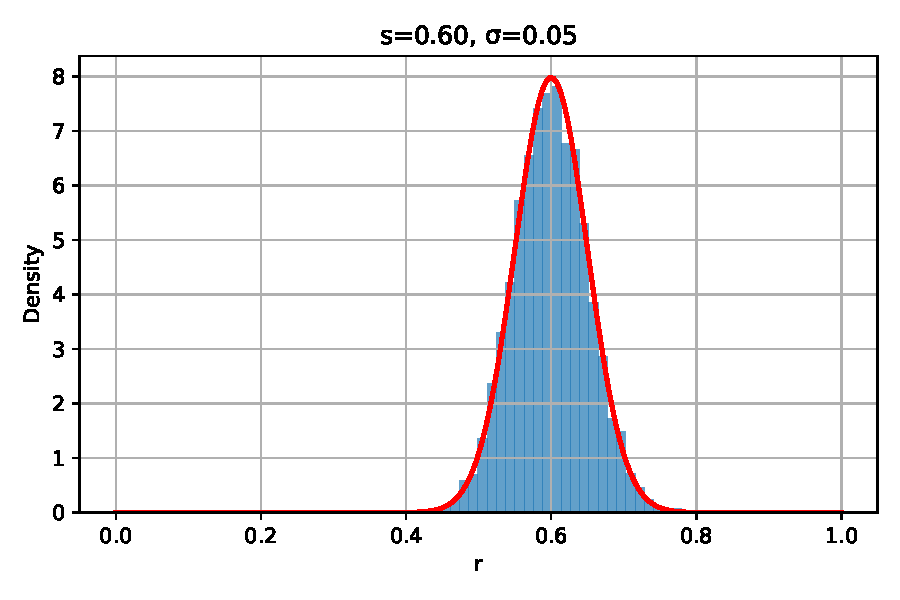
\includegraphics[width=0.32\linewidth]{pics/sampler/s60_step69.pdf} &
    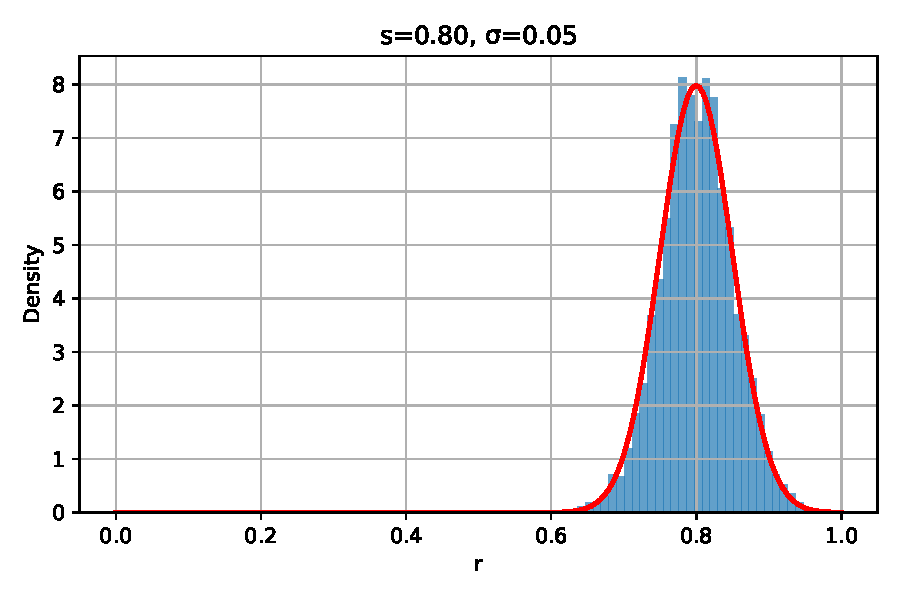
\includegraphics[width=0.32\linewidth]{pics/sampler/s80_step69.pdf} &
    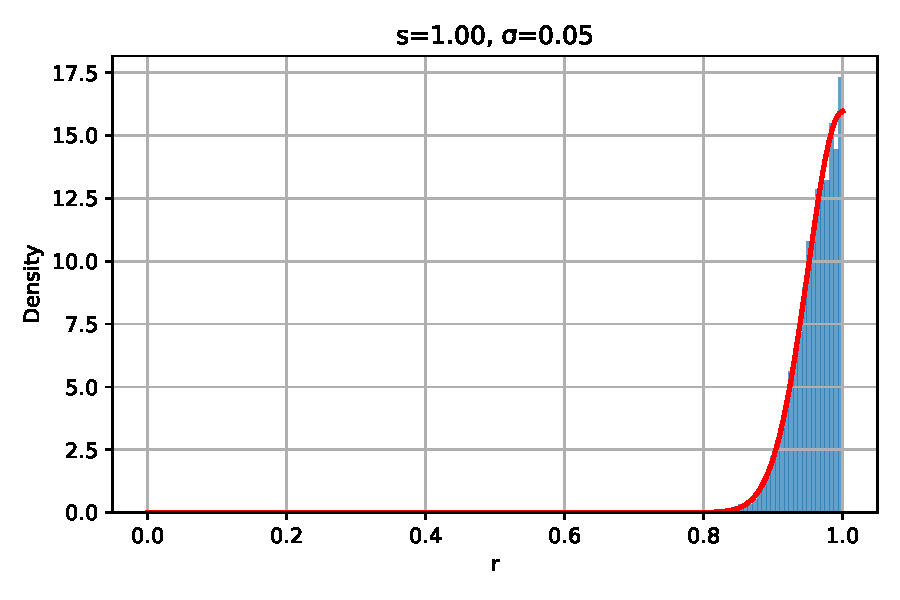
\includegraphics[width=0.32\linewidth]{pics/sampler/s100_step69.pdf} \\
  \end{tabular}
  \caption{Sampling prior \(p(r\mid s)\) on \([0,1]\) for various center values \(s\) with scale \(\sigma=0.05\).}
  \label{fig:trunc_gauss_sigma_0.05}
\end{figure}

%—— figure for σ=0.01 ——%
\begin{figure}[!htbp]
  \centering
  \begin{tabular}{ccc}
    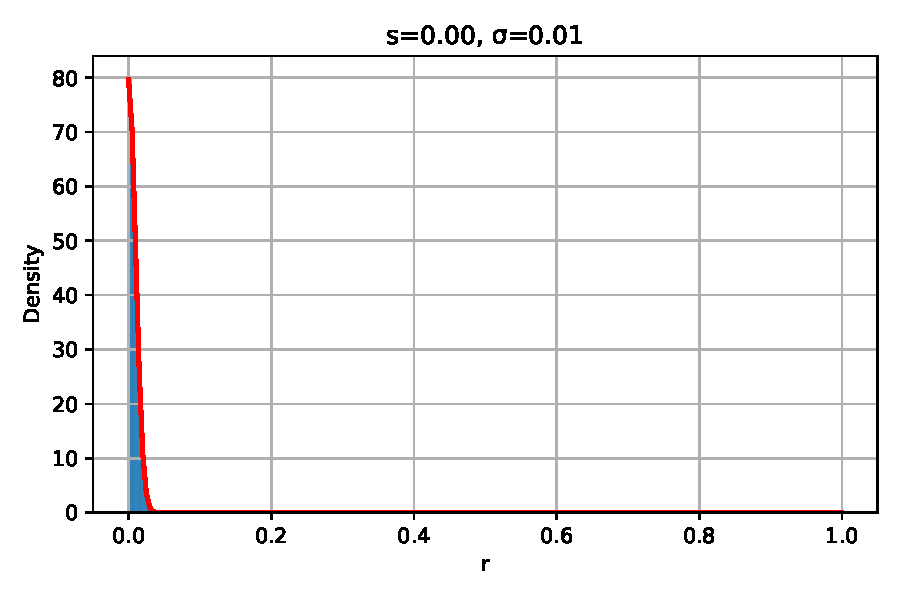
\includegraphics[width=0.32\linewidth]{pics/sampler/s00_step229.pdf} &
    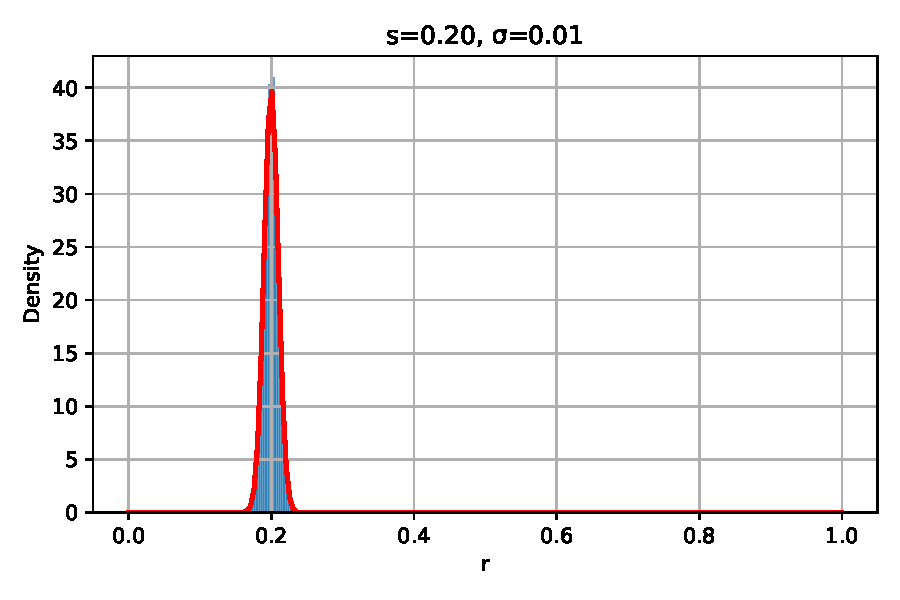
\includegraphics[width=0.32\linewidth]{pics/sampler/s20_step229.pdf} &
    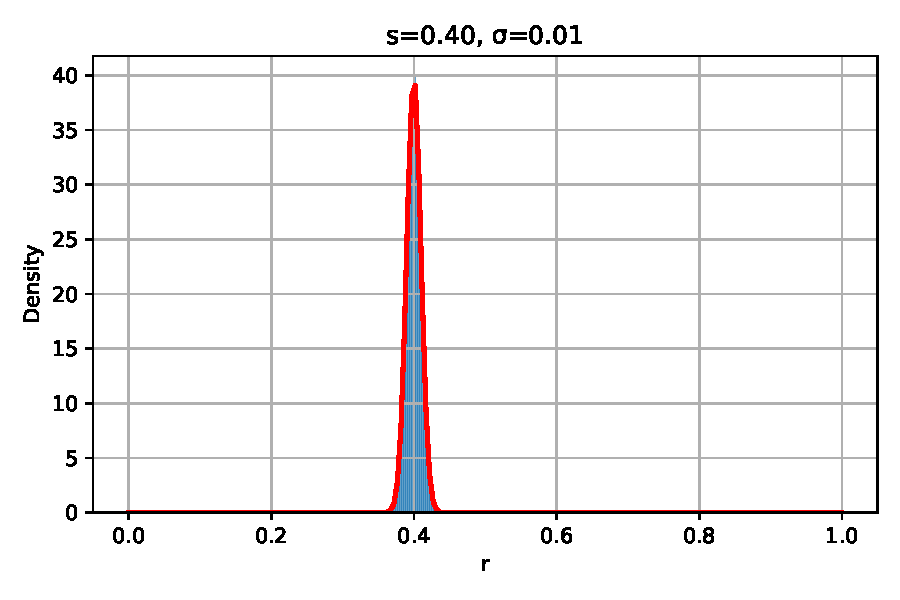
\includegraphics[width=0.32\linewidth]{pics/sampler/s40_step229.pdf} \\
    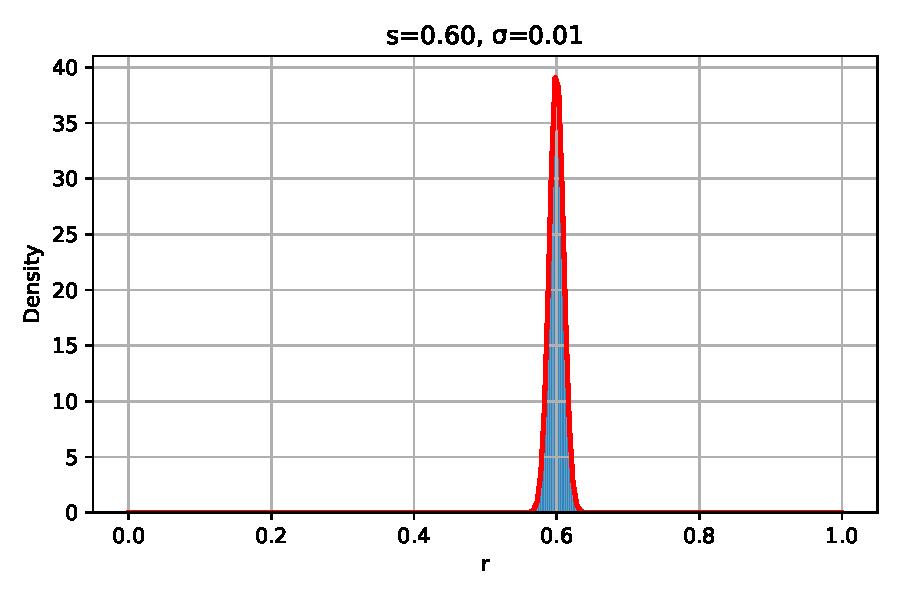
\includegraphics[width=0.32\linewidth]{pics/sampler/s60_step229.pdf} &
    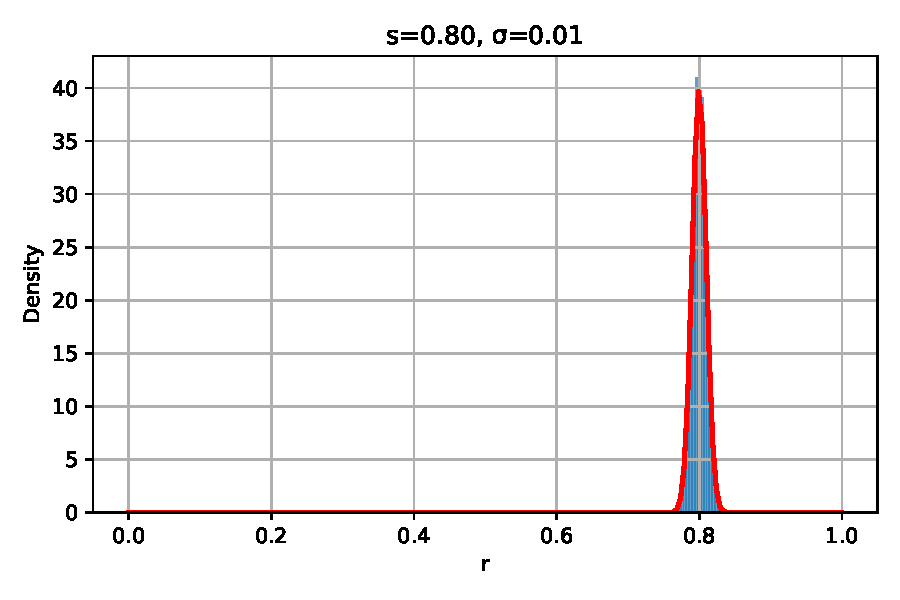
\includegraphics[width=0.32\linewidth]{pics/sampler/s80_step229.pdf} &
    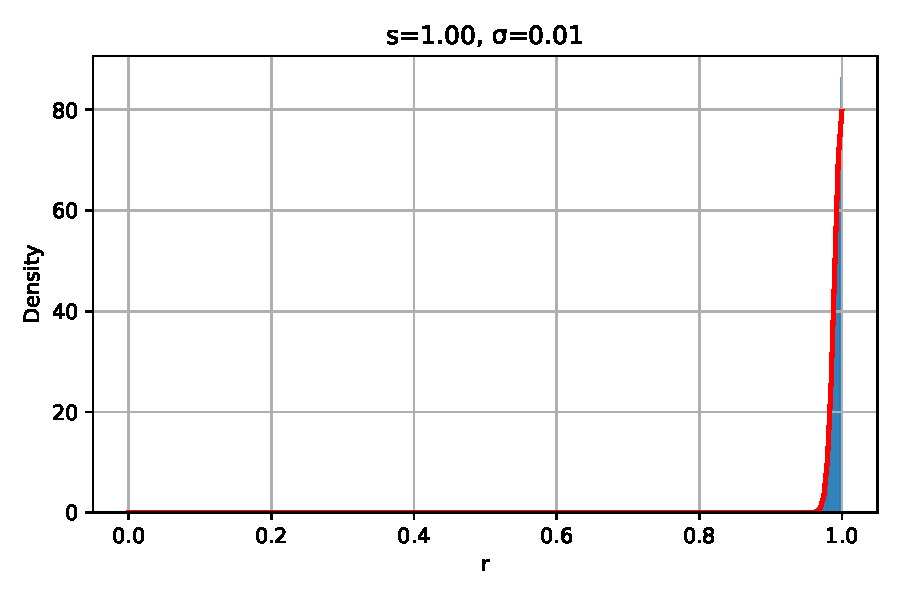
\includegraphics[width=0.32\linewidth]{pics/sampler/s100_step229.pdf} \\
  \end{tabular}
  \caption{Sampling prior \(p(r\mid s)\) on \([0,1]\) for various center values \(s\) with scale \(\sigma=0.01\).}
  \label{fig:trunc_gauss_sigma_0.01}
\end{figure}
